\begin{enunciado}{\ejExtra} \fechaEjercicio{final 19/12/2024}
  Sea $A \en \reales^{n \times n}$ una matriz inversible y sea
  $B =
    \matriz{cc}{
      1 & \bm{c}^t \\
      \bm{b} & A
    }$ con $\bm{b},\, \bm{c}\en \reales^n$.

  \begin{enumerate}[label=\alph*)]
    \item Si $\bm{c} = 0$, probar que $B$ tiene factorización $LU$ si y solo si $A$ tiene factorización $LU$.

    \item Si $\bm{c} \distinto 0$, mostrar que la afirmación del ítem anterior no es verdadera, escribiendo un contraejemplo para ciertos $\bm{b}$, $\bm{c}$
          y $A$ inversible. Justificar.

    \item Si $\bm{c} = 0$, ¿Qué condiciones deben cumplirse sobre $\bm{b}$ y $A$ para que $B$ sea ortogonal?
  \end{enumerate}
\end{enunciado}
% ===============================
% GRAFICOS
% ===============================
\def\bloques{
  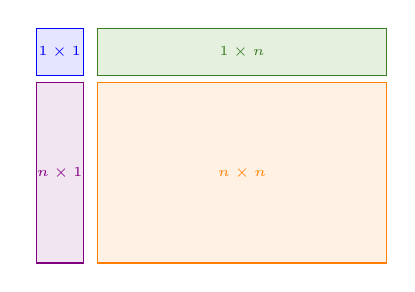
\begin{tikzpicture}[baseline=0, scale = 1.3, every node/.style={font=\tiny}]
    \draw[blue, thin, fill=blue!10,yshift = 0, xshift = -12] (-37px, 20px) rectangle ++(13px,13px) node[midway]{$1\times 1$};
    \draw[OliveGreen, thin, fill=OliveGreen!10,yshift = 0, xshift = -12] (-20px, 20px) rectangle ++(80px,13px) node[midway]{$1\times n$};
    \draw[orange, thin, fill=orange!10,yshift = 0, xshift = -12] (-20px, -32px) rectangle ++(80px,50px) node[midway]{$n \times n$};
    \draw[violet, thin, fill=violet!10,yshift = 0, xshift = -12] (-37px, -32px) rectangle ++(13px,50px)node[midway]{$n \times 1$};
  \end{tikzpicture}
}
\def\bloqueAzul{
  
\begin{tikzpicture}[baseline=10, scale = 0.5, every node/.style={font=\tiny}]
    \draw[blue, thin, fill=blue!10,yshift = 0, xshift = -12] (-37px, 20px) rectangle ++(13px,13px);
  \end{tikzpicture}
}
\def\bloqueAzulZ{
  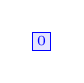
\begin{tikzpicture}[baseline=10, scale = 0.5, every node/.style={font=\tiny}]
    \draw[blue, thin, fill=blue!10,yshift = 0, xshift = -12] (-37px, 20px) rectangle ++(13px,13px) node[midway]{$0$};
  \end{tikzpicture}
}
\def\bloqueVioletZ{
  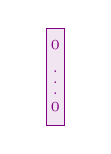
\begin{tikzpicture}[baseline=0, scale = 0.5, every node/.style={font=\tiny}]
    \draw[violet, thin, fill=violet!10,yshift = 0, xshift = -12] (-37px, -32px) rectangle ++(13px,70px)
    node[midway]{$
          \begin{array}{c}
            0      \\
            \vdots \\
            0
          \end{array}
        $
      };
  \end{tikzpicture}
}
\def\bloqueViolet{
  
\begin{tikzpicture}[baseline=0, scale = 0.5, every node/.style={font=\tiny}]
    \draw[violet, thin, fill=violet!10,yshift = 0, xshift = -12] (-37px, -32px) rectangle ++(13px,50px);
  \end{tikzpicture}
}
\def\bloqueVerde{
  
\begin{tikzpicture}[baseline=0, scale = 0.5, every node/.style={font=\tiny}]
    \draw[OliveGreen, thin, fill=OliveGreen!10, yshift = -20, xshift = -12] (-50px, 20px) rectangle ++(80px,13px);
  \end{tikzpicture}
}
\def\bloqueVerdeZ{
  
\begin{tikzpicture}[baseline=0, scale = 0.5, every node/.style={font=\tiny}]
    \draw[OliveGreen, thin, fill=OliveGreen!10, yshift = -20, xshift = -12] (-20px, 20px) rectangle ++(160px,13px) node[midway]{$0 \cdots\cdots\cdots 0$};
  \end{tikzpicture}
}
\def\bloqueOrange{
  
\begin{tikzpicture}[baseline=0, scale = 0.5, every node/.style={font=\tiny}]
    \draw[orange, thin, fill=orange!10,yshift = 0, xshift = -12] (-20px, -32px) rectangle ++(80px,50px);
  \end{tikzpicture}
}
\def\bloqueOrangeZ{
  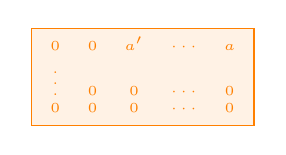
\begin{tikzpicture}[baseline=0, scale = 0.5, every node/.style={font=\tiny}]
    \draw[orange, thin, fill=orange!10,yshift = 0, xshift = -12] (-20px, -32px) rectangle ++(160px,70px)
    node[midway]{
        $
          \begin{array}{ccccc}
            0      & 0 & a' & \cdots & a \\
            \vdots & 0 & 0  & \cdots & 0 \\
            0      & 0 & 0  & \cdots & 0 \\
          \end{array}
        $};
  \end{tikzpicture}
}
% ===============================
% GRAFICOS
% ===============================

\begin{enumerate}[label=\alph*)]
  \item
        \begin{itemize}
          \item[$(\red{\Rightarrow})$] Por hipótesis tengo que $\bm{c} = \bm{0}$ y $B = LU$. El producto en bloques tiene la pinta:
                $$
                  \begin{array}{rcl}
                    B = L \cdot U
                                                                               & =                                                          &
                    \left(\bloques\right)
                    \times
                    \left(\bloques\right)                                                                                                     \\
                                                                               & =                                                          &
                    \matriz{c|c}{
                    \bloqueAzul\ \bloqueAzul + \bloqueVerde\ \bloqueViolet     & \bloqueAzul\ \bloqueVerde + \bloqueVerde\ \bloqueOrange      \\ \hline
                    \bloqueViolet\ \bloqueAzul +  \bloqueOrange\ \bloqueViolet & \bloqueViolet\ \bloqueVerde + \bloqueOrange\ \bloqueOrange
                    }
                  \end{array}
                $$
                $$
                  \ub{
                    \matriz{c|c}{
                      1 & \quad\bm{0}^t \quad \\ \hline
                      &  \\
                      \bm{b} & A\\
                      &
                    }
                  }{
                    B
                  }
                  =
                  \ub{
                    \matriz{c|c}{
                      1 & \quad\bm{0}^t \quad \\ \hline
                      &  \\
                      \bm{d} & \tilde{L}\\
                      &
                    }
                  }{
                    L
                  }
                  \cdot
                  \ub{
                    \matriz{c|c}{
                      1 & \quad\bm{e}^t \quad \\ \hline
                      &  \\
                      \bm{0} & \tilde{U}\\
                      &
                    }
                  }{
                    U
                  }
                  =
                  \matriz{c|c}{
                    1 \cdot 1 + \bm{0}^t \cdot \bm{0} & 1 \cdot \bm{e}^t + \bm{0}^t \cdot \tilde{U}  \\ \hline
                    &  \\
                    \bm{d} \cdot 1 + \tilde{L} \cdot \bm{0}^t  & \bm{d} \cdot \bm{e}^t + \tilde{L} \cdot \tilde{U}  \\
                    &
                  }
                $$

                Donde $\tilde{L}$ y $\tilde{U}$ son triangular inferior y triangular superior respectivamente,
                Para que ese último producto dé $B$, necesito que $\bm{e}^t = \bm{0}^t$ en la primera fila y que $\bm{d} = \bm{b}$ para la
                primera columna.
                Luego obtengo que:
                $$
                  \bm{d} \cdot \bm{0}^t + \tilde{L} \cdot \tilde{U} = A
                  \entonces
                  \cajaResultado{
                    A = \tilde{L}\tilde{U}
                  }
                $$

          \item[$(\red{\Leftarrow})$]
                Para hacer la vuelta tengo la hipótesis de que $A = LU$.
                Dado que $A$ es una matriz inversible y además tiene descomposición $LU$, entonces
                todas las \textit{submatrices esquina}, \textit{submatrices principales}, \textit{sus menores}, son inversibles.

                \parrafoDestacado[\red{\atencion}]{
                  Sea $A \en K^{n \times n}$, \red{$A$ inversible}, entonces:
                  $$
                    A \text{ tiene descomposición } LU \sisolosi
                    \ub{A(1:k,1:k)}{\text{submatrices}\\ \text{principales}}
                    \textit{ es inversible } \paratodo k \en [1,n]
                  $$
                }
                $$
                  B=
                  \begin{tikzpicture}[
                      rect/.style={draw, thin, minimum width=1.2cm, minimum height=1.2cm},
                      submatriz/.style={draw, thin, color=#1, rounded corners=1pt, scale= 0.9},
                      submatriz/.default=red,
                      baseline = 0,
                    ]

                    \matrix (A) [
                      matrix of nodes,
                      nodes={draw = white,
                          rect,
                          anchor=center,
                          font=\small}
                    ] {
                      $\magenta{1}$ & $0$      & $\cdots$ & $0$      \\
                      $\vdots$      & $a_{11}$ & $\cdots$ & $a_{1n}$ \\
                      $\vdots$      & $\vdots$ & $\ddots$ & $\vdots$ \\
                      $\vdots$      & $a_{31}$ & $\dots$  & $a_{nn}$ \\
                    };
                    \node[submatriz=blue, fit=(A-1-1)] {};
                    \node[submatriz=green!70!black, fit=(A-1-1)(A-1-2)(A-2-1)(A-2-2)] {};
                    \node[submatriz=orange, fit=(A-1-1)(A-1-2)(A-1-3)(A-2-1)(A-2-2)(A-2-3)(A-3-1)(A-3-2)(A-3-3)] {};
                    \node[submatriz=violet, fit=(A-1-1)(A-1-2)(A-1-3)(A-1-4)(A-2-1)(A-2-2)(A-2-3)(A-2-4)(A-3-1)(A-3-2)(A-3-3)(A-3-4)(A-4-1)(A-4-2)(A-4-3)(A-4-4)] {};
                    \node[submatriz=black, fit=(A-2-2)(A-2-3)(A-2-4)(A-3-2)(A-3-3)(A-3-4)(A-4-2)(A-4-3)(A-4-4)] {\huge\color{black!20!white}{$A$}};
                    \node[submatriz=black, fit=(A-2-1)(A-3-1)(A-4-1)] {\large\color{black!20!white}{$\bm{b}$}};
                  \end{tikzpicture}
                $$
        \end{itemize}

        Si mirás eso con un poco de amor {\tiny\faIcon{heart}}, vas a notar que las submatrices de $B$ son todas inversibles, dado que sus respectivos determinantes son:
        $$
          \det\big(
          B(1:k,1:k)
          \big) =
          \magenta{1} \cdot
          \ub{
            \det\big(
            A(1: (k-1), 1: (k-1)
            \big)
          }{
            \distinto 0
          }
          =
          A(1: (k-1), 1: (k-1))
          \paratodo k \en [1,n]
        $$
        Es así que si todas las submatrices principales de $B$ son inversibles, entonces:
        $$
          \cajaResultado{
            B \text{ tiene descomposición } LU
          }
        $$

  \item Me armo una matriz $A$ inversible que no tenga $LU$. Y elijo a $\bm{b}$ y $\bm{c} \distinto \bm{0}$
        de forma tal de que tenga en el elemento $[B]_{22} = 0$ y $[B]_{31} = \red{1}$, ese 1 está por debajo de la diagonal de $B$,
        no voy a poder triangular sin permutar.
        $$
          \bm{c}^t = (0 ~ 1 ~ \cdots ~ 1),
          \quad
          \bm{b}^t = (0 ~ 1 ~ \cdots ~ 1),
          \quad
          A =
          \matriz{ccc}{
            \quad & e_{\red{2}} & \quad \\ \hline
            & e_{\red{1}} &  \\ \hline
            & \vdots & \\ \hline
            & e_n &
          }
        $$

  \item Para que $B \en \reales^{(n+1) \times (n+1)}$ sea una matriz ortogonal debe cumplir que $B\cdot B^t = I_{n+1}$
        {\footnotesize
            $$
              \ub{
                \matriz{c|c}{
                  1 & \quad\bm{0}^t \quad \\ \hline
                  &  \\
                  \bm{b} & A\\
                  &
                }
              }{
                B
              }
              \cdot
              \ub{
                \matriz{c|c}{
                  1 & \quad\bm{b}^t \quad \\ \hline
                  &  \\
                  \bm{0} & A^t\\
                  &
                }
              }{
                B^t
              }
              =
              \matriz{c|c}{
                1 \cdot 1 + \bm{0}^t \cdot \bm{0} & 1 \cdot \bm{b}^t + \bm{0}^t \cdot A^t  \\ \hline
                &  \\
                \bm{b} \cdot 1 + A \cdot \bm{0}^t  & \bm{b} \cdot \bm{b}^t + A \cdot A^t  \\
                &
              }
              =
              \matriz{c|c}{
                1  & \bm{b}^t  \\ \hline
                &  \\
                \bm{b}  & \bm{b} \cdot \bm{b}^t + A \cdot A^t  \\
                &
              }
              =
              \ub{
                \matriz{c|c}{
                  1  &\quad \bm{0}^t \quad \\ \hline
                  &  \\
                  \bm{0}  & I_n  \\
                  &
                }
              }{
                I_{n+1}
              }
            $$
          }
        Para que $B$ sea una matriz ortogonal, debe cumplirse que:
        $$
          \cajaResultado{
            \text{$A$ debe ser una matriz ortogonal y $\bm{b} = 0$}
          }
        $$
\end{enumerate}
